\documentclass{sig-alternate}

% some more configurations
%-- Package hyperref ------------------------------------------------------------------------------
\usepackage[
	plainpages=false, %Gibt an auf welcher Seite die pdf-Darstellung beginnt.
	pdfpagelabels,
	pdftex=true,
	breaklinks=true, %/false: Gibt an, ob Links umgebrochen werden duerfen.
	%linktocpage=true/false: im Inhaltsverzeichnis sind nur die Seitenzahlen links, nicht der Text
	colorlinks=true, %/false: Links werden eingefaerbt (Farben werden mit linkcolor, anchorcolor ... festgelegt)
	linkcolor=black, %Farbe des verlinkten Textes, Dokument-interne Links
	citecolor=black, %Farbe des verlinkten Textes, Links zum Literaturverzeichnis
	filecolor=black, %Farbe des verlinkten Textes, Links auf lokale Dateien
	urlcolor=black, %Farbe des verlinkten Textes, externe URLs
	%frenchlinks=true/false: Links werden als smallcaps, anstatt farbig dargestellt.
	menucolor=black
]{hyperref}

\hypersetup{
	pdftitle={GreenSubway},
	pdfauthor={Andreas Jahn, Stephan Sigg},
	pdfsubject={GreenSubway},
	pdfkeywords={GreenSubway},
	%pdfpagelayout={TwoColumnRight}
	%bookmarksnumbered=true,
	%bookmarksopen=true,
	%bookmarksopenlevel=1,
	%pdfpagemode=None % None, UseOutline, UseThumbs, FullScreen
}
\usepackage{balance}  % to better equalize the last page

\begin{document}

\title{The Foretelling Subway: Environment and Situation}

\numberofauthors{2} %  in this sample file, there are a *total*
% of EIGHT authors. SIX appear on the 'first-page' (for formatting
% reasons) and the remaining two appear in the \additionalauthors section.
%
\author{
% You can go ahead and credit any number of authors here,
% e.g. one 'row of three' or two rows (consisting of one row of three
% and a second row of one, two or three).
%
% The command \alignauthor (no curly braces needed) should
% precede each author name, affiliation/snail-mail address and
% e-mail address. Additionally, tag each line of
% affiliation/address with \affaddr, and tag the e-mail address with \email.
%
% 1st. author
\alignauthor
Andreas Jahn and Klaus David\\
       \affaddr{Kassel University}\\
       \affaddr{Wilhelmh\"oher Allee 73}\\
       \affaddr{Kassel, Germany}\\
       \email{\{andreas.jahn,david\}@uni-kassel.de}
% 2nd. author
\alignauthor
Stephan Sigg and Xiaoming Fu\\
       \affaddr{Goettingen University}\\
       \affaddr{Goldschmidtstr. 7}\\
       \affaddr{G\"ottingen, Germany}\\
       \email{\{stephan.sigg, fu\}@informatik.uni-goettingen.de}
% 3rd. author
% \alignauthor
% Klaus David\\
%        \affaddr{Kassel University}\\
%        \affaddr{Wilhelmh\"oher Allee 73}\\
%        \affaddr{Kassel, Germany}\\
%        \email{david@uni-kassel.de}
}

% Title
\maketitle

% Abstract
\begin{abstract}
In this work we introduce the environment for passenger occupancy prediction
\end{abstract}

% Introduction
\section{Introduction}
\label{sec:introduction}

Underground transportation systems are big energy consumers and have significant impacts on energy consumptions at a regional scale~\cite{anderson_maximizing_2009}. 

So far the optimization of the energy efficiency of transportation equipments, e.g. trains have been considered. Optimization of the energy efficiency of the metro stations operations, however, is only minimally exploited.

But realizing savings in energy consumption are meaningful for two reasons:
(\textit{i})~Despite the relatively small percentage that can be gained with optimal management of one metro station compared to optimizing trains, the high numbers of metro stations in the underground transportation will yield large energy savings in overall terms. In other words, in the management of metro stations is a high multiplication factor that boosts each relative small saving at a station level to a high saving at a metro network level.
Moreover (\textit{ii}) the optimization of the energy efficiency of the metro stations involves much less investments than the ones that are usually applied to transportation means and equipments. Consequently is it possible to distributed the technology easily across the whole metro network, as well as other transportation systems and realize savings in short term.

For example all Barcelona (Spain) metro stations consumes 63,1 millions of kWh annually~\cite{TMB}. A relative small saving of, e.g. 5\% in the electricity consumption of one metro station, is equivalent to the electricity consumed in more than 700 households during one year.

The optimized management of stations and surroundings, such as ventilation, vertical transportation and lighting does have an impact.

An approach to optimize the energy efficiency and to realize energy savings is to
enable the station to control the surroundings, such as ventilation, vertical transportation and lighting "intelligent" according the current situation. 
A simple example of "intelligent" control could be the slowing down the frequency of the ventilation-fans of the station, when the count of passenger doesn't make full speed necessary.

To achieve the context aware behaviour of a metro station basically two parts are necessary. (i) A controller which calculate the appropriate actions. A controller which is adaptive on the basis of various environmental factors, forecasts and passenger occupancy was developed~\cite{guo_intelligent_2013}.
(ii) The environmental factors, and prediction must be available for the controller. 

Staying in the given example the controller needs be aware about the current count of passengers in order to decrease the fan frequency if possible. However, increasing the fan frequency is more complex. Since the decreasing of the fan frequency doesn't have an immediate effect for the air quality the fan frequency needs to be decreased in a appropriate time before the stations is abruptly crowed again. To guarantee the required air quality on every point in time, the ventilation needs to be controlled in a foreseen manner, i.e. controlled on the prospectively number of passenger in the station.

This paper presents an approach for predicting the prediction of number of passenger in the station.

The remainder of this paper is organized as follows. In Section~\ref{sec:stateOfTheArt} an overview of the related literature is given. Section~\ref{sec:dataAcquisition} focuses on the data acquisition and the experiments, followed by Section~\ref{sec:results}, the evaluation and results. Last, Section~\ref{sec:conclusion}, summarizes the results.


% Test Environment & Station
\section{Environment}
\label{sec:Environment}

\subsection{SEAM4US}
\label{subsec:seam4us}

% TODO
The seam4us project...

The prediction is based on occupancy data gathered in a metro station. Following the environment were the research takes place, i.e. the metro station is described more in detail.

\subsection{Underground Station Passeig de Gr\`{a}cia}
\label{subsec:station}

In this section the "station" is described. First the word "station" in the area of metro networks needs to be defined.

A metro network is composed by one or more metro lines. Each line has a fixed railway with a given number of stops to allow people to get on or off the trains by means of a platform: each of these stops is called "line station". A "metro station" is the concept that represents the point in space through which a passenger gets underground and into a line station. Metro station and line station can be the same physical entity, but it is possible that there are some "metro stations" that receive two or more "metro lines" in different platforms, and have therefore, two or more "line stations" within.

The data, used in this work, are gathered in line station in Passeig de Gr\`{a}cia - Line~3~(PdG-L3) in Barcelona. Passeig de Gr\`{a}cia~(PdG) is a station in the metro network of "Transports Metropolitans de Barcelona"~(TMB) and lies in a very iconic and touristic part of Barcelona. Some of the most popular buildings designed by Antoni Gaudi are in the proximity (Casa Batll\`{o}, Casa Mil\`{a}), as well as the city's most renown and exclusive boutiques.
The metro station is a historic icon of the Barcelona metro network. First opened in December of 1924, as a (line) station for Line~3, nowadays PdG holds three different line stations: L2, L3, and L4. The stations were built in three different periods and using different construction technologies in each of the premises (contemporary to the building periods). All line stations station has been refurbished a few times since 1924 and new equipment has been added recently.

Depending on the weekday PdG is open 19~hours, 21~hours or 24~hours. Between Monday and Thursday PdG service starts at 5:00 and ends at 24:00 (19~hours). Friday service starts at 5:00 and ends at 2:00 (21~hours). On Saturday service starts at 5:00 to but remain the entire night until midnight on Sunday.

Passeig~de~Gr\`{a}cia - Line~3~(PdG-L3) turns out to be representative for many station within TMBs metro network~\cite{TMB}. Moreover PdG-L3 is a crowded station which have low-rate usage hours as well. This provides a wide range of data which allows to test with very busy peak hours as well as with off-peaks. Figure~\ref{fig:PdG-L3_platforms} depicts the platforms of PdG-L3.

\begin{figure}[htb]
  \centering
  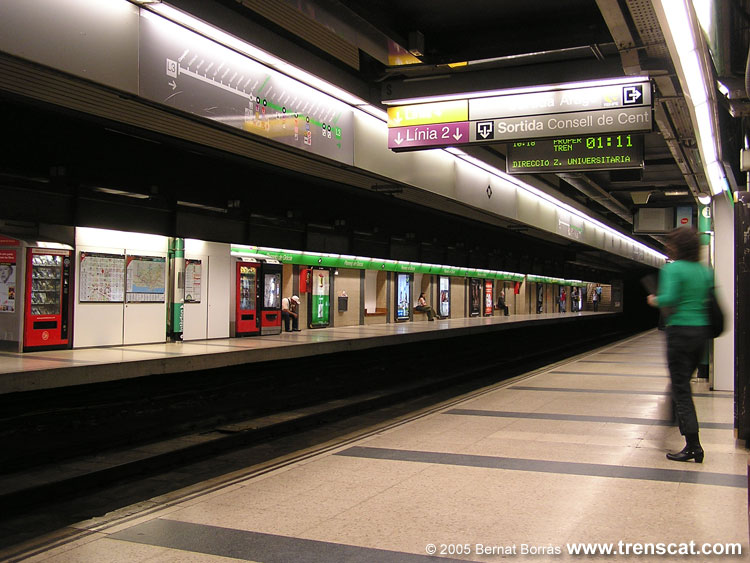
\includegraphics[width=\linewidth]{Figures/PdG-L3_platforms.jpg} 
  \caption{PdG-L3 Plattforms. \cite{TMB}}
  \label{fig:PdG-L3_platforms}
\end{figure}

The line station PdG-L3 consists of several public spaces: halls, transit areas, accesses to the platforms, and platforms. Furthermore there are private spaces such as technical rooms or staff dependencies. The private spaces are not part of the investigation in this work. Figure~\ref{fig:PdG-L3_schematic} depicts the line station schematic where the accesses to platforms are highlighted in red.

\begin{figure}[htb]
  \centering
  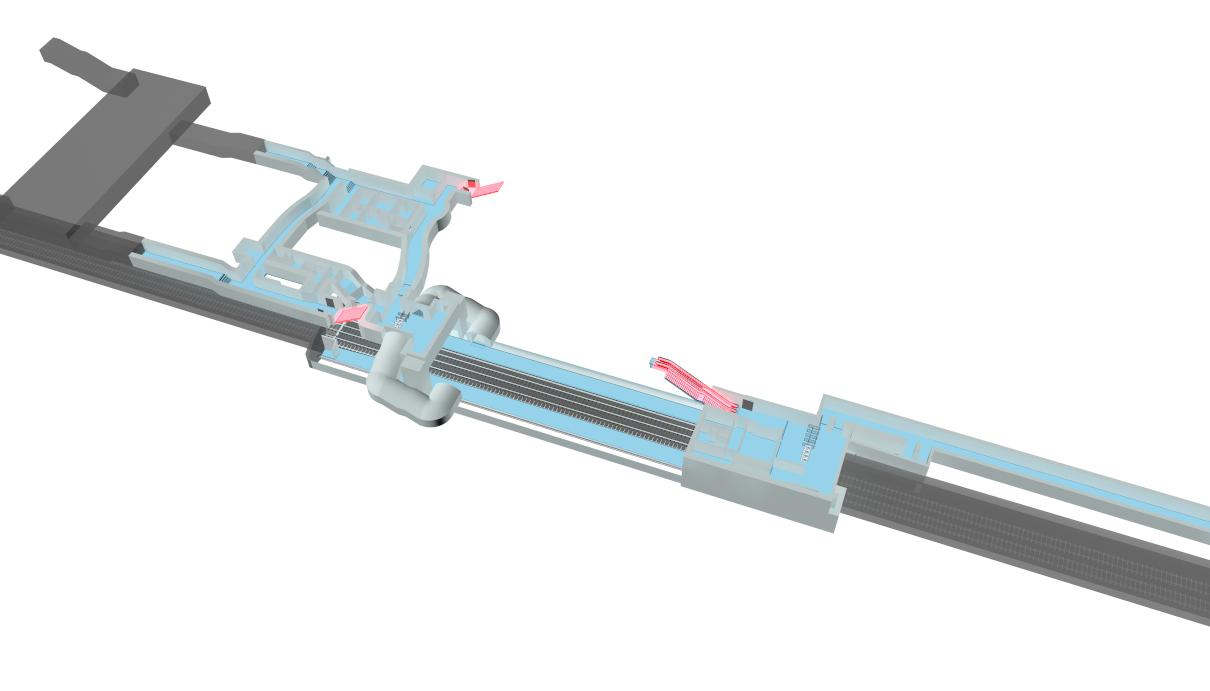
\includegraphics[width=\linewidth]{Figures/PdG-L3_schematic.jpg} 
  \caption{Schematic representation of PdG-L3. The accesses to platforms are highlighted in red. \cite{TMB}}
  \label{fig:PdG-L3_schematic}
\end{figure}

The public spaces are equipped with a Closed Circuit Television~(CCTV) for security reasons. The cameras of the CCTV-system provide images which contains the information how many people are on a dedicated time on a dedicated place. To gather these information the images needs to be processed. In the following the processing of the CCTV images is described in short.


\subsection{Passenger density data}
\label{subsec:PassengerDensityData}

Whenever the camera pictures are processed the privacy issues are tackled. To ensure the privacy restrictions several actions took place.
First of all, all CCTV images needed for prediction purposes does not leave the station. To ensure this, the image processing is conducted on a dedicated computer especially bought for this purpose. The PC is located in technical room within the station. The images are just for "on the fly" image processing and are not stored on the PC.
All information 

Throughout the station a CCTV surveillance system already exists. 22~CCTV~cameras are in place where each camera provides in a circuit design subsequently the images. The images provided by each CCTV-camera are stored on a video recorder. A crowd density estimator processes the images and returns the number of passengers on this image. The number of passenger as well as date, time and the camera-ID are saved in a database.

For different reasons, e.g. bad camera picture or network errors it is possible that the image processing fails. In this case the image processing return the error value "-1".

The process images are not saved for privacy reasons. Figure~\ref{fig:CCTVimageProcessing} depict the processing chain.

\begin{figure}[htb]
  \centering
  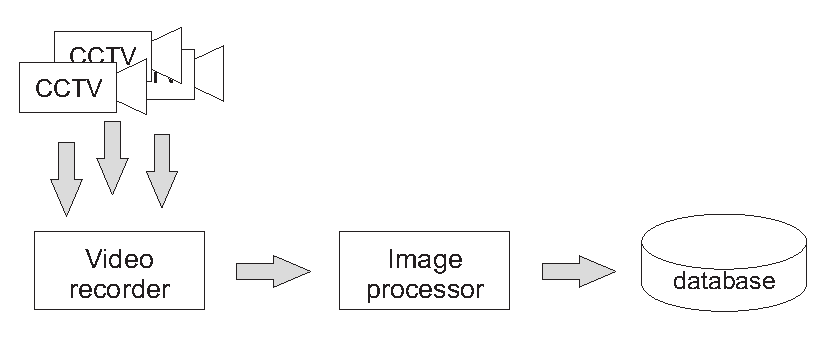
\includegraphics[width=\linewidth]{Figures/imageProcessing.pdf} 
  \caption{Gathering number of people out of the camera images.}
  \label{fig:CCTVimageProcessing}
\end{figure}

The CCTV and image processing runs 24~hours, 7~days a week. Each day 31680~datasets are saved to the database. Overall the database contains 90~days of data.
Figure~\ref{fig:rawData_week} illustrates exemplary the available values of a week. At a more detailed view of a day the service times are visible (Figure~\ref{fig:rawData_day}).

% one column
\begin{figure*}[tb]

  \centering

  \subfigure[Passenger density distribution of one camera during one week.] {
    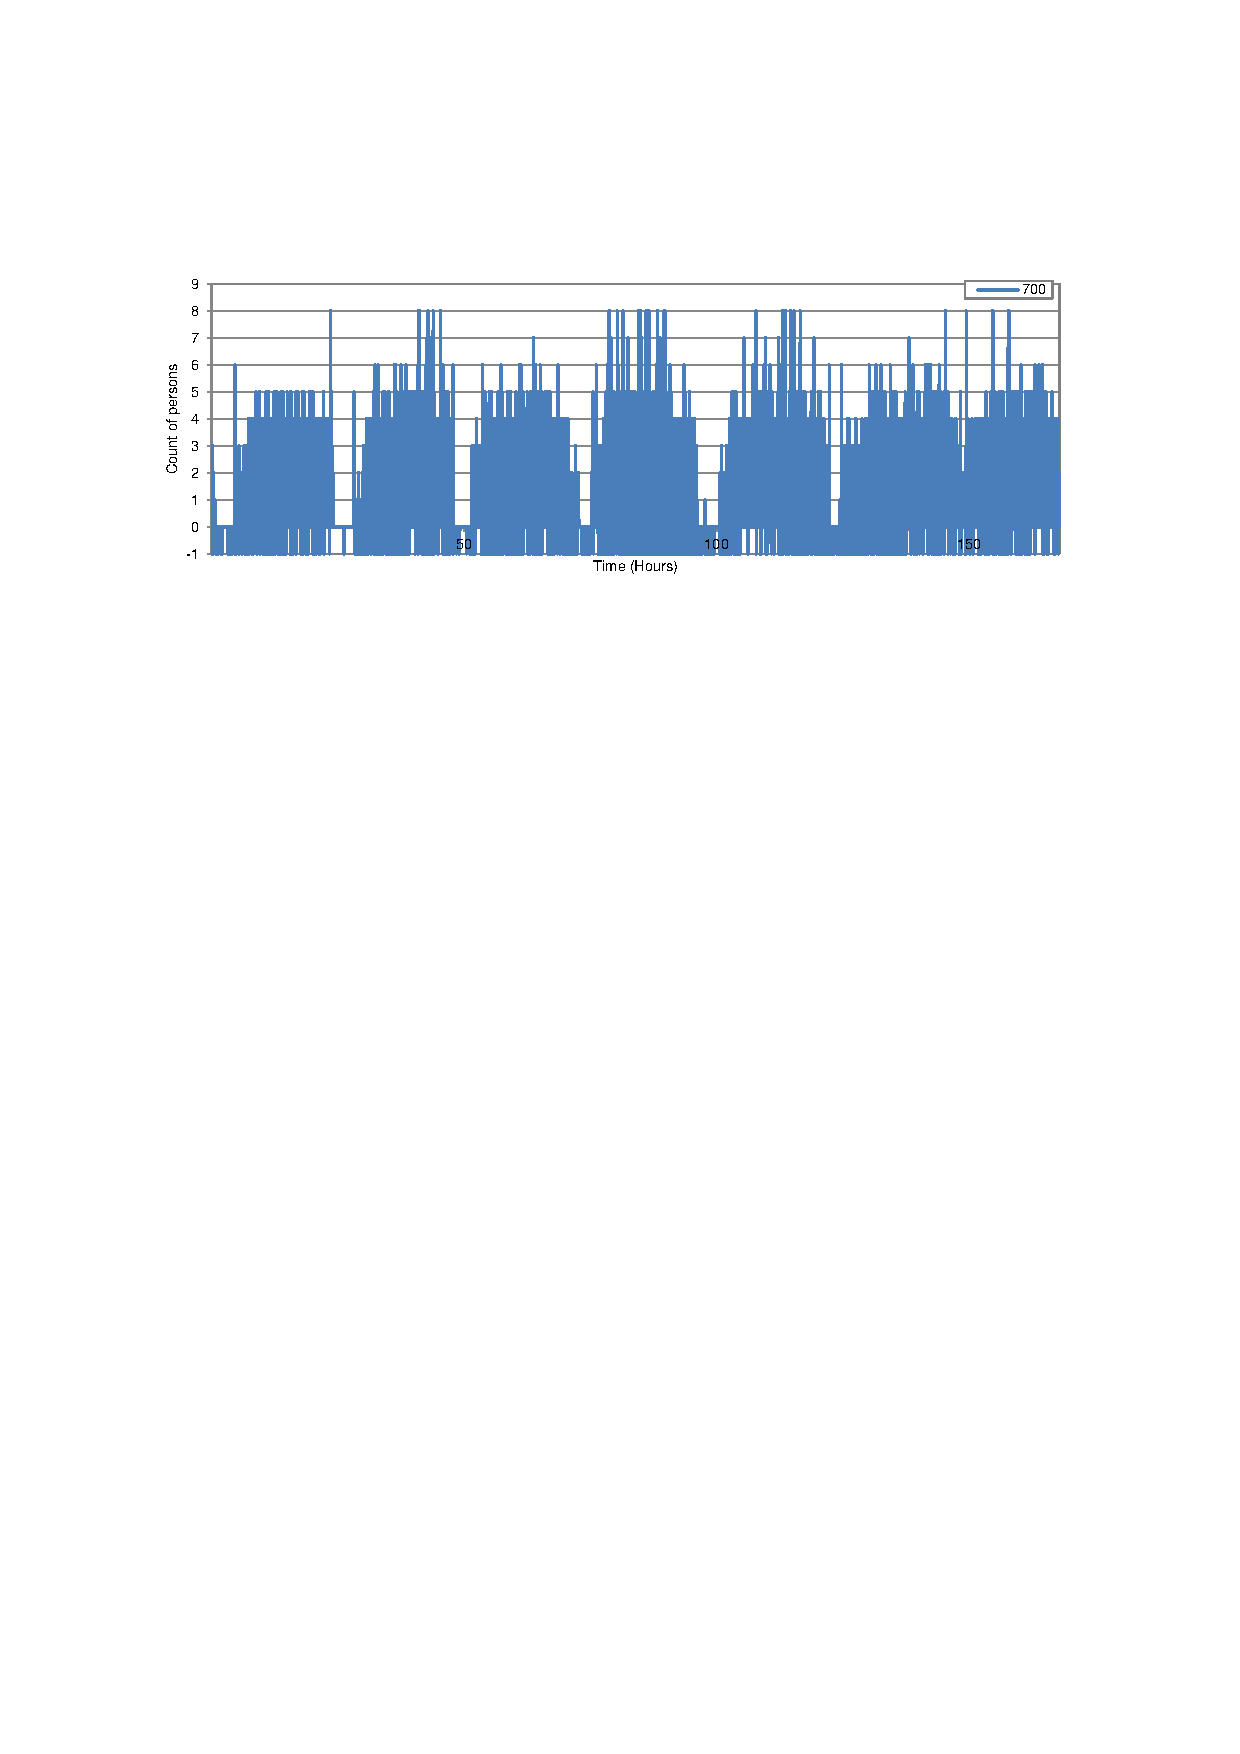
\includegraphics[width=0.46\textwidth]{Figures/rawData_week.pdf}
    \label{fig:rawData_week}
  }
  \hfill
  \subfigure[Passenger density distribution of one camera during one day.] {
    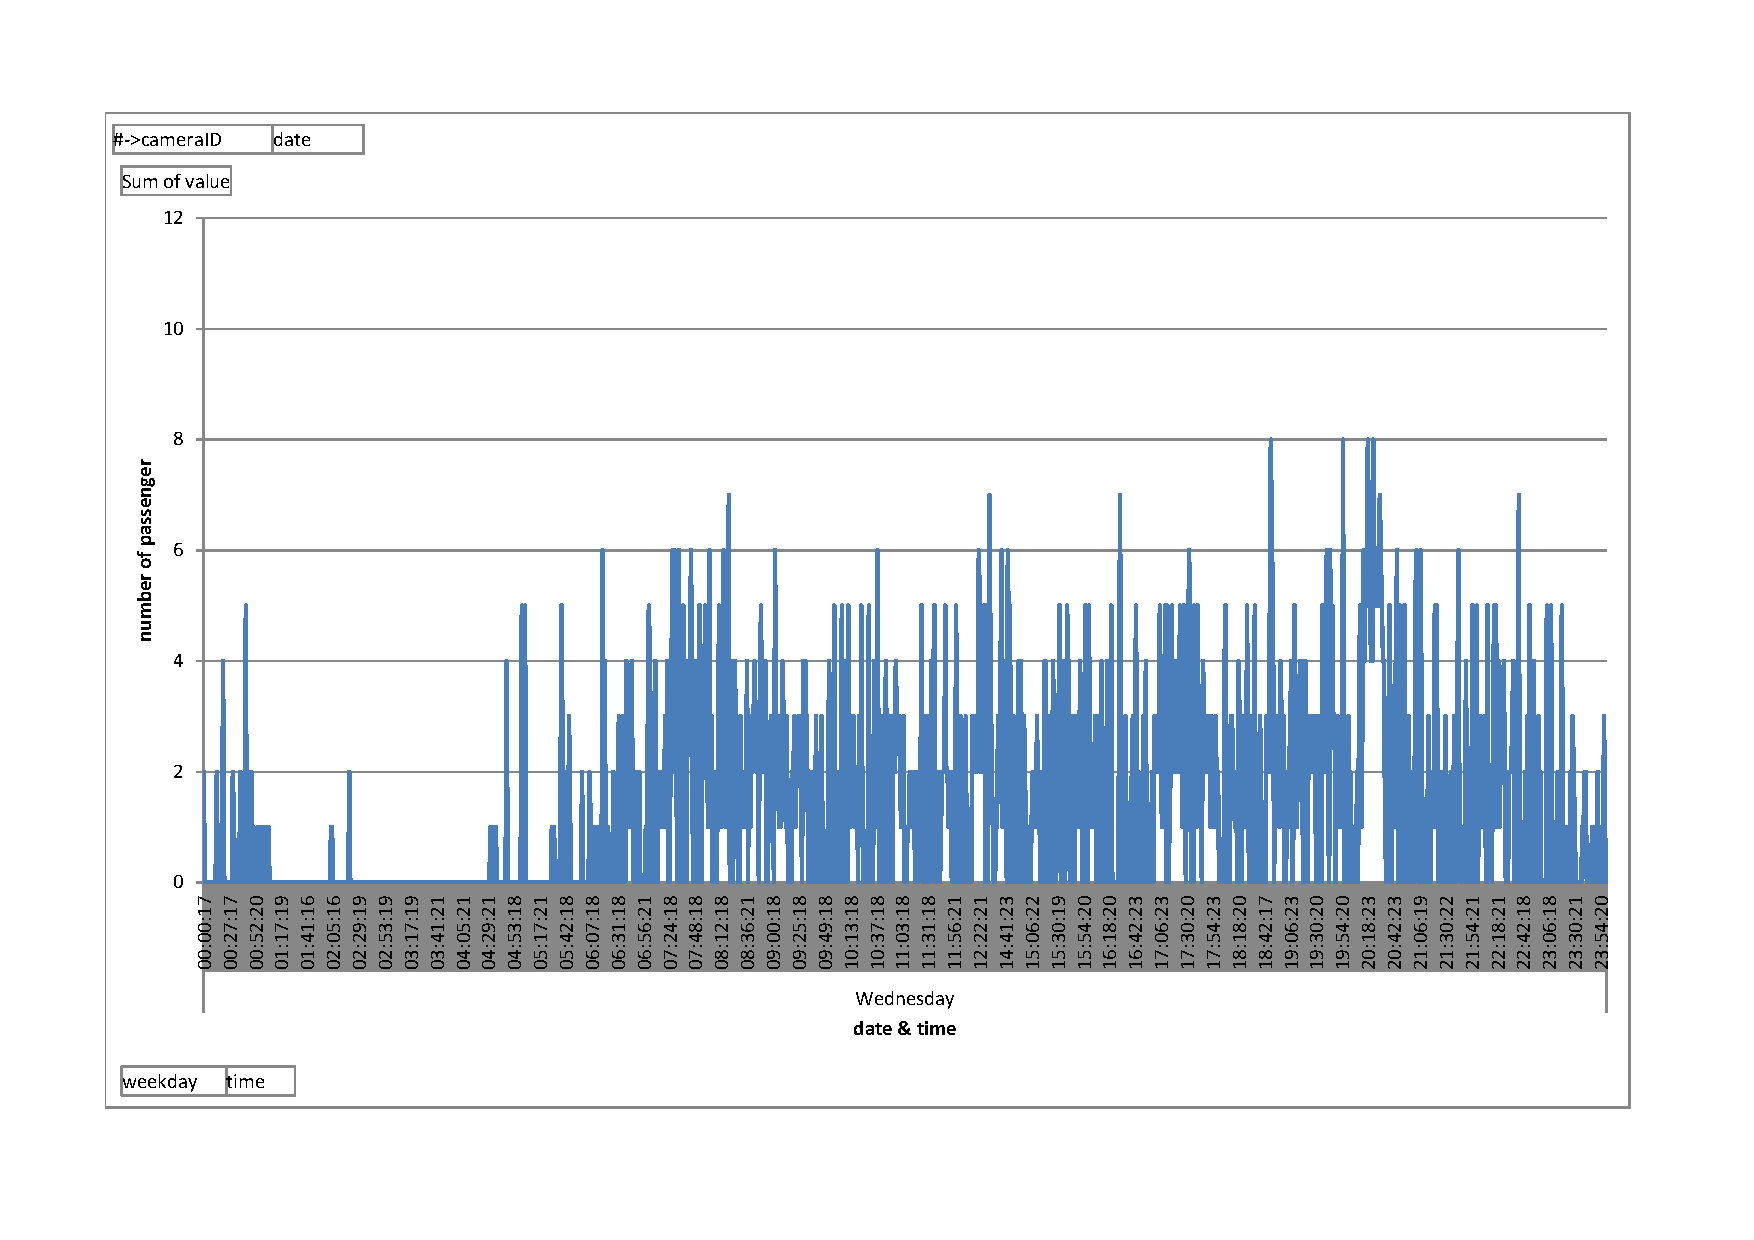
\includegraphics[width=0.46\textwidth]{Figures/rawData_day.pdf}
    \label{fig:rawData_day}
  }

  \caption{Passenger density distribution of one camera.~\cite{TMB}.}
  \label{fig:rawData}

\end{figure*}



% Conlusion
\section{Conclusion}
\label{sec:conclusion}

Conclusion


\let\oldtocsubsection=\tocsubsection
% Acknowledgements
\section{Acknowledgements}
\label{sec:acknowledgements}

This work was partially funded by the EU-FP7 project "Sustainable Energy mAnageMent 4(for) Underground Systems" (SEAM4US, FP7-ICT, EEB-ICT-2011.6.4). The authors would like to acknowledge the contributions of their colleagues.

\balance

% References
\label{sec:references}
\bibliography{references.bib}
\bibliographystyle{plain} %alpha plain


\end{document}